%%%%%%%%%%%%%%%%%%%%%%%%%%%%%%%%%%%%%%%%%
% Friedrich M. Grabner - 01220997
% Masters Project Report
%%%%%%%%%%%%%%%%%%%%%%%%%%%%%%%%%%%%%%%%%

%----------------------------------------------------------------------------------------
%	PACKAGES AND DOCUMENT CONFIGURATIONS
%----------------------------------------------------------------------------------------

\documentclass{beamer}
\usepackage{graphicx} % Required for the inclusion of images
\usepackage{multicol}
\graphicspath{{./images/}}

\setbeamertemplate{navigation symbols}{}
\usetheme{Singapore}
\beamersetuncovermixins{\opaqueness<1>{25}}{\opaqueness<2->{15}}

%----------------------------------------------------------------------------------------
%	BEGIN DOCUMENT
%----------------------------------------------------------------------------------------
\begin{document}
\setbeamertemplate{footline}[text line]{\parbox{\linewidth}{\vspace*{-8pt}\centering Imperial College London}
}
\title{\huge{HPC on the Cloud}} 
\author{Author: Friedrich Grabner\\
Supervisor: Dr C. Cantwell}
\date{\today} 

\begin{frame}
\titlepage
\end{frame}

\section{Introduction} 
\begin{frame}\frametitle{Introduction}
\textbf{Context:}
\begin{itemize}
\item Advancements in computing power has increased the feasibility of high-order numerical simulation to solve complex engineering problems.
\item Availability to IaaS systems has allowed those outside large institutions to gain access to high performance computing.
\end{itemize}
\textbf{\color{red}{Problem:}}
\begin{itemize}
\item Nevertheless many people still prefer to use low-order commercial software, on personal hardware.
\end{itemize}
\end{frame}

\begin{frame}\frametitle{Introduction}
\textbf{Why do people prefer commercial codes?}
\begin{itemize}
\item Complex and daunting interface of open-source softwares.
\item High-level of expertise required to understand how to run properly run a simulation. (numerical methods, submitting jobs, post-processing)
\item Lack of support for users.
\end{itemize}
\end{frame}

\begin{frame}\frametitle{Nekkloud and TemPSS}
\begin{itemize}
\item  Nekkloud is a web based platform through which the Nektar solvers can be launched.
\item Nekkloud streamlines the running of simulations through access to IaaS systems.
\item TemPSS provides the graphical user interface for Nekkloud, from which to instantiate input files for Nektar.
\end{itemize}
\centering
\vspace{3pt}
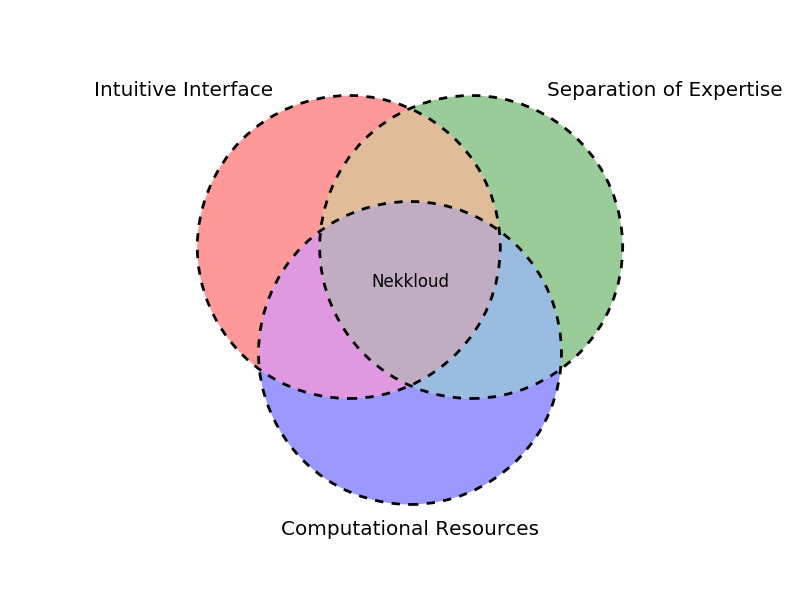
\includegraphics[width=.75\linewidth,  clip=true, trim = 0cm 0cm 0cm 2cm]{venn_diagram}
\end{frame}


\begin{frame}\frametitle{Aims and Objectives}

\textbf{Objectives:}
\begin{enumerate}
\item Map functionality within the incompressible flow solver.
\item Understand and detail the constraints between said functions.
\item Develop TemPSS transform templates that instantiate all functions.
\item Represent these functions and constraints within an intuitive interface.
\item Perform a beta testing of the interface with Nektar users and implement recommendations.
\item Test the operation of XML generation, through benchmarking against a selection of representative testcase.
\end{enumerate}
\end{frame}

\section{Methods and Theory}
\begin{frame}\frametitle{Methods} 
Each frame should have a title.
\end{frame}

\begin{frame}\frametitle{Constraints} 
\href{http://localhost:8081/nek_dep.html}{\beamergotobutton{Interactive Constraints Visualiser}}
\end{frame}

\begin{frame}\frametitle{TemPSS Incompressible Navier-Stokes} 
\href{http://localhost:8081/nek_dep.html}{\beamergotobutton{Interactive Constraints Visualiser}}
\end{frame}

\section{Conclusion}
\begin{frame}\frametitle{Conclusions} 
Each frame should have a title.
\end{frame}

\begin{frame}\frametitle{Future Work and Recommendations} 
Each frame should have a title.
\end{frame}

\end{document}